\section{Smart $\alpha$ Scheduler}
\label{sec:alpha-approach}

As a first dynamic chunk size approach we propose \algalpha, \ie a scheduling algorithm, which dynamically adjusts the chunk size $s$ based on measured throughput and latency changes similar to how TCP handles link congestion. 
In~\xref{sec:background-tcp}, the necessary TCP background knowledge in flow- and congestion-control is explained to fully understand our approach. 

The key idea is that when a link is loosing in quality TCP will adjust the server's sending rate and this might result in a change of the throughput rate at the \mhttp~client. 
When measuring the throughput rate at the client over time we can detect these changes and adjust our chunk size accordingly, thus taking advantage of TCP's optimized link quality estimates. 

In the following we introduce our algorithm for two active connections for simplicities sake, but the algorithm can be easily converted to the scenario that involves more than two connections.

Let $c_1$ and $c_2$ be the connections established by \mhttp. 
We denote by $\overline{R}_i$ and $\overline{rtl}_i$ the estimated throughput and latency (round trip) of $c_i$, and by $s_{i,j}$ the size of the $j$th chunk to be transmitted over $c_i$. 
In~\xref{sec:metrics} we explain in more detail how $\overline{R}_i$ and $\overline{rtl}_i$ are estimated. 

We determine the chunk size $s_{i,j}$ through:

$$s_{i,j}=\alpha_i \cdot \overline{rtl}_i \cdot \overline{R}_i$$

$\alpha_i$ is a value that adjusts based on the evolution of the throughput $\overline{R}_i$. 
This approach is very similar to TCP's congestion window adjustments as discussed in~\xref{sec:background-tcp}. 
Basically $s_{i,j}$ is $\alpha_i$ multiples of bytes that are estimated to be received during $\overline{rtl}_i$. 

We introduce $\alpha_{init}, \delta_{inc}$ and $\delta_{dec}$, which are chosen experimentally and will influence how $\alpha_i$ increases or decreases over time. 
Currently, $\delta_{inc}$ and $\delta_{dec}$ are set to $2$ and $0.9$ respectively. 
The optimal values for these two variables need to be investigated closer in further mobility studies as discussed in~\chref{ch:discussion}.

Given a series of throughput measurements $R_i(t)$, where $t=0,1,\cdots,n-1$, 
we use a Linear Increase / Multiplicative Decrease approach in order to slowly increase and quickly decrease $\alpha_i$, meaning 
$\alpha_i$ is increased linearly by $\delta_{inc}$ if the currently measured throughput $R_{i}(n)$ is sufficiently larger\footnote{Sufficiently means larger than $\gamma \cdot R_{i}(n-1)$, where $\gamma=1.01$} than the previously measured value $R_{i}(n-1)$ or was already decreased in the previous calculation. 
In any other case $\alpha_i$ is multiplicatively decreased by $\delta_{dec}$. 
Through the use of a \term{DECREASED} Flag the algorithm avoids two consecutive decreases in a row, thus an endless decrease spiral is impossible, since after every decrease at least one increase needs to occur. 
Note, that our prototype does not support request pipelining yet which results in a certain idle time between receiving payload blocks.
The \term{DECREASED} Flag is important, since due to wrong estimates we might otherwise schedule very small chunks, which results in more idle times and might decrease the overall sender rate. 
When bad link quality occurs, it is still possible for the scheduler to decrease to a very small chunk size though, since multiplicative decrease evolves faster than linear increase.

We summarize the calculation of $\alpha_i$ in~\alref{alg:dynamic-alpha}.

\begin{algorithm}
\caption{\algalpha~Algorithm}
\label{alg:dynamic-alpha}
\begin{algorithmic}
\STATE{Init: $DECREASED \gets FALSE$}
\STATE{$\gamma \gets 1.01$}
\STATE{$\delta_{dec} \gets 0.9$}
\STATE{$\delta_{inc} \gets 2$}
\IF{$n = 0$}
	\STATE{$\alpha_i \gets \alpha_{init}$}
\ELSE
	\IF{$\gamma \cdot R_{i}(n-1) < R_{i}(n)$ \OR $DECREASED$}
		\STATE{$\alpha_i \gets \alpha_i + \delta_{inc}$}
		\STATE{$DECREASED \gets FALSE$}
	\ELSE
		\STATE{$\alpha_i \gets \delta_{dec} \cdot \alpha_i$}
		\STATE{$DECREASED \gets TRUE$}
	\ENDIF
\ENDIF
\end{algorithmic}
\end{algorithm}

One thing to consider when using this approach is that TCP starts with a very small congestion window, meaning the full capacity of the link is not used initially. 
As already mentioned there exists a certain idle time between receiving payload blocks. 
It follows that if our requested chunk sizes are very small, the TCP congestion window might not grow to its full potential and thus we would waste throughput performance. 
Hence, it is desirable to keep the $\alpha$ value relatively high and to not choose $\alpha_{init}$ too small.

Further, note that the very first chunk over a new connection $c_i$ has a predefined initial chunk size of $32$KB. 
This is due to the fact that initially we have no link estimates yet. 
After receiving this initial chunk we have link quality estimates to make better decisions. 

\begin{figure*}[t]
		\begin{minipage}[t]{0.5\linewidth}
		\begin{center}
                \subfigure[Chunk size evolution of \algalpha.]{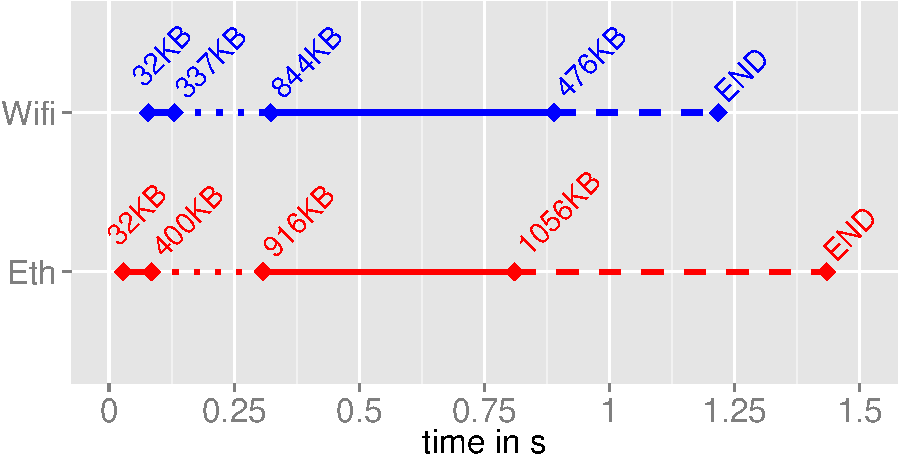
\includegraphics[width=\linewidth]{Figures/flow-dynamic-alpha.pdf}}
        \end{center}
        \end{minipage}
~
        \begin{minipage}[t]{0.5\linewidth}
        \begin{center}
                \subfigure[Chunk size evolution of \algslice.]{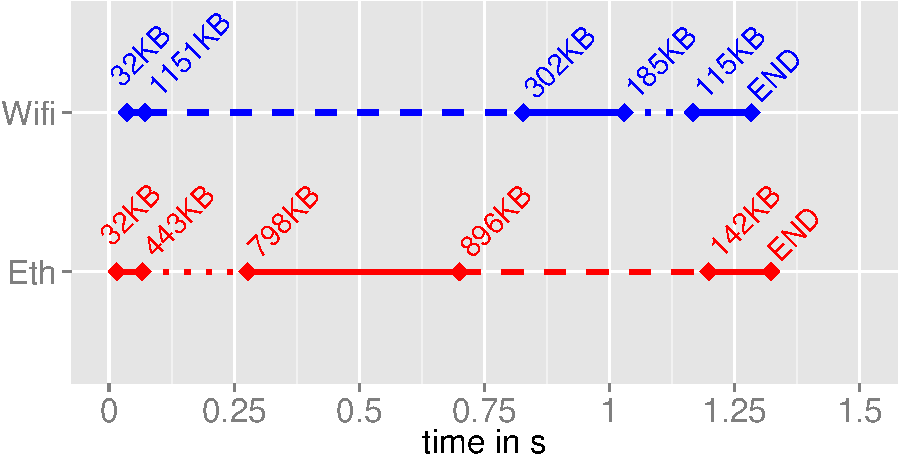
\includegraphics[width=\linewidth]{Figures/flow-dynamic-slices.pdf}}
        \end{center}
        \end{minipage}
        \caption{\label{fig:scheduler-flows} Illustrative examples of how the chunk sizes evolve in case of a $4$MB file download with the \algalpha~scheduler (a) and with the \algslice~scheduler (b).}
  \vspace*{-0.3cm}
\end{figure*}

In~\fref{fig:scheduler-flows} (a) we see an illustrative example of how the chunk sizes evolve on a $4$MB file download with the \algalpha~scheduler. 
We can see how the chunk sizes are getting bigger shortly after the initial chunks, since our throughput estimates are rising and more accurate. 
The first chunk for each connection is the predefined initial chunk size of $32$KB. 
Later the difference between the chunk sizes of each connection is due to the different measured link qualities. 
We can also clearly see that the last chunk of the \wifi~connection is much smaller than the previous one. 
This is due to the fact that we reached the end of the file and there are no more chunks to request. 
This example illustrates very good that we successfully achieve a variable chunk size based on the link quality. 
Moreover, it illustrates an essential problem that still needs to be solved, \ie in the end the \wifi~connection stays idle for a relatively long time. 
It is desirable to synchronize the last chunk download of each connection to avoid such idle times. 
In~\xref{sec:synchronization-approach} we propose an algorithm that solves this problem. 
